\todo[inline]{Incomplete}
First, we provide a pre-processing step with the objective of having a segmented
point  set  of  the object  \ref{sec:pre}.  This  is  then  used to  create  the
probabilistic shape representation \ref{sec:object}. This is then exploited in

%%%%%%%%%%%%%%%%%%%%%%%%%%%%%%%%%%%%%%%%
\subsection{Object Segmentation}
\label{sec:segmentation}
\todo[inline]{To review, complete todos}

As stated in Secs.~\ref{sec:equipment}~and~\ref{sec:limitations}, a partial point cloud
of a segmented object is required in order to get observation points for the initial
surface estimation and speed up the shape modeling.
\citet[Sec.~III.A]{Hudson2012Endtoend}  provides  good   candidate algorithms  for  object
segmentation  that are  well oriented  to  object grasp,  manipulation, and  for
our  purposes, exploration.  In fact,  the  combination of  their ``Table  Plane
Estimation''  with their  ``Volume-Based  Segmentation''  yields the  ubiquituos
tabletop object segmentation \citep{TabletopObjectDetector}. However, to improve
the  rechability  of the  exploration,  we  prefer to  hold  the  object in  one
hand-arm system and explore with the other, as described in Sec.~\ref{sec:scope}.
\todo[]{Descrition in section 3 is missing. Also should point to the subsection, not the section.}
Thus,  our selected  approach  for  object segmentation  is  simpler than  those
approaches.  The  difficulties are  in  measuring  the  configuration of  a  soft
and  adaptable  hand, like the Pisa/IIT SoftHand,
\todo[]{I think we should cite some softhand paper here.}
that  keeps  the  object  in  position  to  filter  out
the  points  belonging  to  the  hand-arm system.  For  this  purpose,  one  can
rely in  body-type measurements  instead of  traditional encoders,  as described
in~\citet{Santaera2015Lowcost}.
\todo[inline]{i think we need to tell also that we are using an imu glove for the softhand,
    but there's no paper about the glove yet. So what!?}
Once the hand-arm  system pose is measured, then
some   passthrough filters with slightly  scaled bounding boxes of  the robot
geometry  are used  to obtain  a  point cloud  of  the object  isolated from  the
robot. The scaling factor $\kappa$ is used to account for any incertainties that might
be present in the robot state or in the point cloud measurements. 
By slightly enlarging the robot bounding boxes we make sure that the object is correctly
separated from it, at the cost of losing some object points on the hand-object edge.

A further box filter is then applied to isolate the object from the rest of the scene,
thus obtaining a segmented object point cloud. 
Finally the obtained point cloud is further resampled to reduce the overall point
density, maintaing the object geometrical properties, while at the same time
improving Gaussian Process computation speed. 
\todo[]{Perhaps voxel grid description can be omitted}

This last downsampling step is performed with a Voxel Grid Filter, which, after
building a grid of voxels on top of the point cloud, it
substitutes all points in a voxel with their centroid, thus reducing the total number of 
points, while maintaining the object geometrical properties intact. The final desired
point cloud resolution can be controlled with $\delta$ parameter, which is just the edge length of each voxel.
Fig.~\ref{fig:in-hand-segmentation} shows the procedure applied to a real scene,
while  Algorithm~\ref{alg:in-hand-segmentation} resumes  the whole  procedure in
the pseudo-code.

\begin{algorithm}[h]
    \textbf{$\mathcal{O} \leftarrow$ \textsc{segmentInHand}}($\mathcal{P}$, $\mathcal{R}$, $\kappa$, $\delta$)\\ %functionname
\LinesNumbered
\DontPrintSemicolon
\SetAlgoVlined \SetKwInOut{Input}{input} \SetKwInOut{Output}{output}
\Input{The complete scene point cloud, $\mathcal{P}$, the robot model, $\mathcal{R}$, its visual geometry inflation factor, $\kappa$, and the downsampling resolution, $\delta$.}
\Output{The segmented object point cloud, isolated from the scene, $\mathcal{O}$.}
  $\mathbf{r} \leftarrow$\textsc{robotState}($\mathcal{R}$) \\
  $\mathcal{B} \leftarrow$\textsc{boundingBoxes}($\mathcal{R}$, $\mathbf{r}$, $\kappa$) \\
  $\mathcal{O^\prime} \leftarrow$\textsc{passtroughFilters}($\mathcal{P}$, $\mathcal{B}$) \\
  $\mathcal{O} \leftarrow$\textsc{downsampleFilter}($\mathcal{O^\prime}$, $\delta$) \\
  \Return{$\mathcal{O}$}
\caption{In-hand object segmentation.} \label{alg:in-hand-segmentation}
\end{algorithm}

The \textsc{robotState}($\cdot$) method retrievs istantaneous joint states
of the whole hand-arm system ($\mathbf{r}$), which is used by \textsc{boundingBoxes($\cdot$)} to compute robot bounding boxes ($\mathcal{B}$)
from its geometrical properties, known by the robot model ($\mathcal{R}$).

\textsc{passtroughFilters}($\cdot$) repeatedly performs filters to remove
all points found inside the hand-arm system bounding boxes, obtaining $\mathcal{O^\prime}$.
That is finally resampled with the desired resolution ($\delta$) 
to obtain the final segmented object ($\mathcal{O}$), in \textsc{downsampleFilter}($\cdot$) function.

\todo[inline]{rewording-removal?}
It is worth noting, that this procedure is here also to show how visual and tactile
data might  be merged into a  single shape model.
But,  as a matter of  fact, the
initial training  point set  can be  empty and the whole shape modeling could be 
started  by simply  probing naively towards the gripper.

\begin{figure}
\centering
  \mbox{
  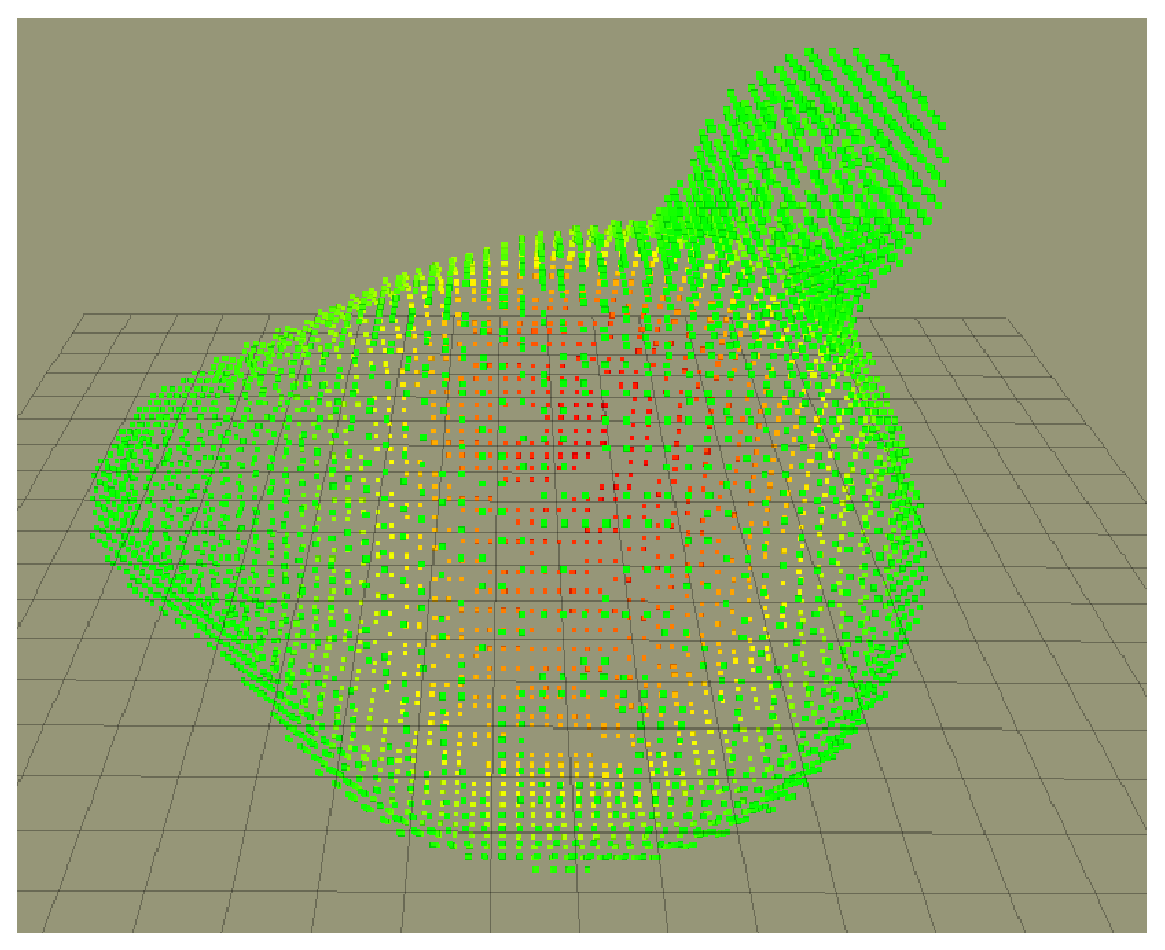
\includegraphics[width=0.45\linewidth]{example.eps}
  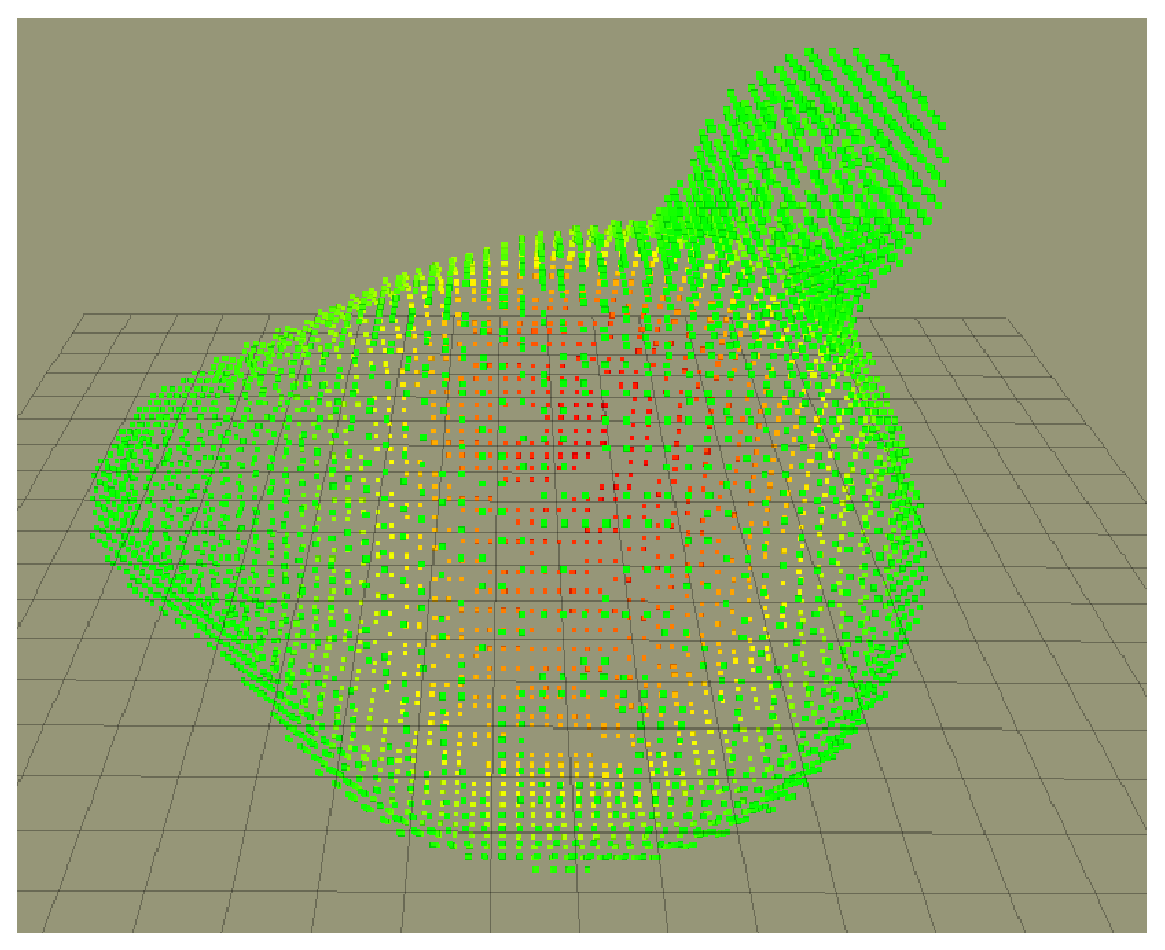
\includegraphics[width=0.45\linewidth]{example.eps}
  }
  \caption{A picture of the in-hand object segmentation using a soft-adaptive hand on a 7-dof arm in the real scene (left) and the resulting point cloud (right).}
  \label{fig:in-hand-segmentation}
\end{figure}



%%%%%%%%%%%%%%%%%%%%%%%%%%%%%%%%%%%%%%%%
\subsection{Shape modelling}
\label{sec:shape}
\todo[inline]{To write}
What makes a good surface representation?
\begin{itemize}
\item Accurate (we handle this with probability)
\item Concise (we might want this)
\item Intuitive specification (we don't need this)
\item Local support
\item Affine invariant 
\item Arbitrary topology (we need this)
\item Guaranteed continuity (we need this)
\item Natural parameterization (we don't need this)
\item Efficient display (we shouldn't need this)
\item Efficient intersections (we could need this)
\end{itemize}

Looks like implicitly defined surfaces are the best...

How do we define implicit function?
\begin{itemize}
\item Algebraics
\item Blobby models
\item Skeletons
\item Procedural
\item Samples
\item Variational
\item Gaussian Process !
\end{itemize}

Variational surfaces:
\begin{itemize}
\item Advantages:
\begin{itemize} 
\item Easy to test if point is on surface
\item Easy to compute intersections/unions/differences
\item Easy to handle topological changes
\end{itemize}
\item Disadvantages:
\begin{itemize}
\item Indirect specification of surface
\item Hard to describe sharp features
\item Hard to enumerate points on surface !
\item Slow rendering !
\end{itemize}
\end{itemize}

Except from rendering and surface explicit related things... but we don't actually need that except from debug.

\begin{figure}
\centering
  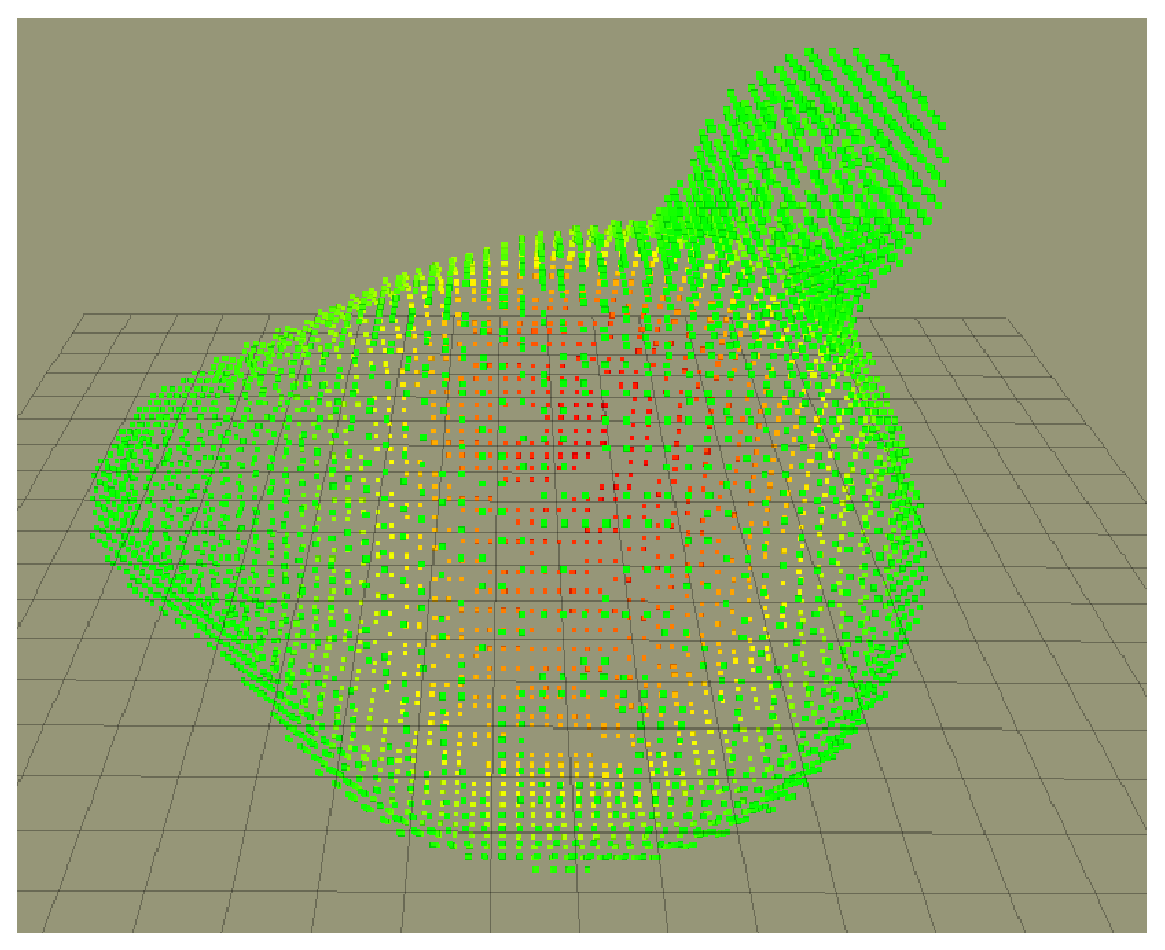
\includegraphics[width=0.9\linewidth]{example.eps}
  \caption{Different shape representations} \label{fig:shape-comparison}
\end{figure}

\begin{algorithm}[h]
\textbf{\textsc{createGaussianProcess}}($X$)\\ %functionname
\LinesNumbered
\DontPrintSemicolon
\SetAlgoVlined \SetKwInOut{Input}{input} \SetKwInOut{Output}{output}
\Input{The training data, $\mathcal{X}$, in the form of a point cloud.}
\Output{The Gaussian Process that models the object shape.}
  $\mathcal{D} \leftarrow$\textsc{deMeanNormalizeAndLabel}(\{$\mathcal{X}$, $\mathbf{0}_{\text{sizeOf}(\mathcal{X})}$\}) \\
  \textsc{addLabeledPoint}(\{$\mathbf{0}_3, -1\}$, $\mathcal{D}$) \\
  \textsc{addLabeledPoints}(\{\textsc{sphere}$(\mathbf{0}_3, 1.1, N)$, $+\mathbf{1}_{N}\}$, $\mathcal{D}$) \\
  $\mathcal{G} \leftarrow$ \textsc{doRegression}($\mathcal{D}$) \\
  \Return $\mathcal{G}$ \\
\caption{Gaussian Process regression} \label{algo:strategy}
\end{algorithm}

%%%%%%%%%%%%%%%%%%%%%%%%%%%%%%%%%%%%%%%%
\subsection{Exploration strategy}
\label{sec:strategy}
\todo[inline]{F: needs some reviewing, but looks like a decent draft to me :)}
\todo[inline]{Notation conflict}

% We don't need all the conditions described in \citet[Fig.~8]{Jaillet2013Path}.
The exploration strategy, employs  the concept of Rapidly-exploring Random Trees to build
an Atlas on  the Gaussian Process surface. Then  it decides which
is  the  best next  tactile  action  to perform  in  order to improve the  current
object shape estimation.

This is achieved by an RRT explorer, called $\mathcal{T}$, who's in charge
of progressively build a tree of interconnected elements, or nodes,  until a termination criterion is met.
Conceptually the object $\mathcal{T}$ behaves similarly to a classical RRT planner,
but it does not have a goal to pursue, it just needs to explore the surface widely
enough in order to tell where the next tactile action should take place, so that
the estimated surface uncertainty is reduced the most.
For this reason we called $\mathcal{T}$, the RRT explorer and not planner even if
both objects are conceptually very similar.

The RRT explorer, however does not have any information on the model on which is built, specifically,
it just need to track the connections between nodes of the tree and decide where it
should expand next. All the model information is stored in an Atlas, called $\mathcal{A}$.

An atlas can be viewed as a collection of maps or charts and conceptually it is able
to create new charts at a given location on the surface it is currently modelling.
Furthermore $\mathcal{A}$ is able to expand a given chart, producing new locations
from where create new charts.

In the proposed exploration strategy, RRT nodes are exactly the atlas charts, thus
building such a tree is like composing an atlas, which tries to model the implicit
estimated surface.

Formally we define a chart $\mathcal{C}$ with a center point on the surface $\mathbf{x}_{c}$,
such that
$$
\mathbb{E}(\mathcal{S}(\mathbf{x}_c)) \approx 0
$$
with a search space defined as a
tangent disc at the surface, centered on $\mathbf{x}_c$, with radius 
$$
R \propto \frac{1}{\mathbb{V}(\mathcal{S}(\mathbf{x}_c))}
$$ 
and finally with the gradient information at the center 
$$
G \approx \frac{\partial \mathcal{S}}{\partial \mathbf{x}}
$$
Conventionally the center variance is addressed as the chart variance, because
it locally approximates the uncertainty of the surface estimation.

With such charts, the atlas can be defined as the set of all charts plus some parameters
responsible for chart creation:
$$
\mathcal{A} \triangleq \{\mathcal{C}_1, \ldots, \mathcal{C}_i, \ldots, \mathcal{C}_n, \Omega^{\mathcal{A}}\}
$$
where $n$ is the number of created charts and $\Omega^{\mathcal{A}}$ are the parameters.

The explorer can also be viewed as a collection of chart connections, or branches,
plus another set of parameters responsible for the tree expansion behaviour:
$$
\mathcal{T} \triangleq \{\mathcal{C}_i \leftarrow \mathcal{C}_j, \ldots, \Omega^{\mathcal{T}}\}_{i \neq j \le n}
$$

With such tools, the exploration strategy can be summarized by Algorithm~\ref{alg:strategy}.
\begin{algorithm}[h]
    \textbf{$\mathcal{P} \leftarrow$ \textsc{exploreGPAtlasRRT}}($\mathcal{M}$, $\Omega$)\\ %functionname
\LinesNumbered
\DontPrintSemicolon
\SetAlgoVlined \SetKwInOut{Input}{input} \SetKwInOut{Output}{output}
\Input{A Gaussian Process model, $\mathcal{M}$ and the set of parameters $\Omega$, defining criteria
    to decide how to start, extend and end the exploration.}
\Output{The best next action, $\mathcal{P}$, in the form of a path, if any, or $\varnothing$ otherwise.}
$\mathcal{A}, \mathcal{T}, \mathbf{x}_{c,i} \leftarrow$\textsc{init}($\mathcal{M}$, $\Omega$) \\
$\mathcal{C}_{i} \leftarrow$\textsc{create}($\mathcal{A}$, $\mathbf{x}_{c,i}$, $\Omega$)\\
  \While{ \textsc{notTermination}($\mathcal{C}_{i}$, $\Omega$)}
  {
    $\mathcal{C}_{j} \leftarrow$\textsc{select}($\mathcal{T}$, $\Omega$) \\
    $\mathbf{x}_{c,k} \leftarrow$\textsc{expand}($\mathcal{A}$, $\mathcal{C}_{j}$, $\Omega$) \\ 
    $\mathcal{C}_{k} \leftarrow$\textsc{create}($\mathcal{A}$, $\mathbf{x}_{c,k}$, $\Omega$) \\ 
    \textsc{connect}($\mathcal{T}$, $\mathcal{C}_{k}$, $\mathcal{C}_{j}$) \\
    $\mathcal{C}_{i} = \mathcal{C}_{k}$ \\
  }
  \eIf {\textsc{solution}($\mathcal{C}_{i}$)}
  {\Return $\mathcal{P} \leftarrow$\textsc{path}($\mathcal{C}_{i}, \mathcal{T}$)}
  {\Return $\varnothing$}
  \caption{Best-next tactile action strategy} \label{alg:strategy}
\end{algorithm}

Given a Gaussian Process model, $\mathcal{M}$, approximating the implicit object surface
with a regression, as described in Sec.~\ref{sec:gpr}, and the set of parameters
$$\Omega \triangleq \Omega^{\mathcal{A}} \cup \Omega^{\mathcal{T}}$$
An empty atlas and a RRT explorer can be initialized.
Then a starting point is selected randomly among the object training set:
$$
\mathbf{x}_{c,i} \in \chi^0
$$
where $\chi^0$ is the set of object points,
which in turn is part of the Gaussian Process Model, $\mathcal{M}$.

$\mathcal{A}$ is charged to create the first chart, also called \emph{root}, from the starting point,
then the algorithm rapidly builds the tree of charts on the object until the supplied termination
criterion is met, or the maximum allowed number of charts has been reached.
The best-next tactile action is finally the path from the converging chart to the root, or nothing if no such chart exists.

The main loop of the algorithm is fulfilled by the following steps:\\
\begin{inparadesc}
\item[select($\cdot$)] Ask the explorer to select a chart to expand,
among the chart collection ($\mathcal{A}$).
This is done by selecting one at random with a bias to increase the probability
of selecting the last created chart. This criterion is adopted to grow a tree
which is more inclined to expand on a single branch, but at the same time maintain the
possibility to create new branches from previous charts. So efficiency and speed
is preserved, while we make sure we are exploring as much surface as possible,
before reaching a solution.\\
\item[expand($\cdot$)] The selected chart $\mathcal{C}_j$ is expanded by $\mathcal{A}$, by
sampling $k$ points on its tangent discs then selecting one at maximum variance
and at the same time not in collision with other charts search spaces. 
So a sample $\mathbf{s}_i$ is selected if 
$$
\mathit{max}_{i\in k}[\mathbb{V}(\mathcal{S}(\mathbf{s}_i))]
$$
and 
$$
{\parallel\mathbf{s}_i - \mathbf{x}_{c,j}\parallel}_{2} > R_j, \forall \mathcal{C}_j \in \mathcal{A}_{i \ne j}
$$
where $\mathbf{x}_{c,j}$ is the center and $R_j$ is the tangent disc radius of $\mathcal{C}_j$.

The selected $\mathbf{s}_i$ is then projected back on the surface,
creating a center for a new chart, $\mathbf{x}_{c,k}$.
The projection is performed with a gradient descend method, using the gradient estimation
of the chart $G_j$.\\
\item[create($\cdot$)] A new chart  is created on the projected point, maintaining the atlas
    expansion on the estimated implicit surface
$$
\mathcal{C}_k \in \mathcal{A}
$$
\item[connect($\cdot$)] creates a connection to the chart which originated the newly created one,
    drawing a new branch for the tree
$$
\{\mathcal{C}_j \leftarrow \mathcal{C}_k \} \in \mathcal{T}
$$
\end{inparadesc}

$\mathcal{C}_k$ is then tested for the termination condition and the whole loop
starts anew.

The progressively growing tree of charts expands on the object surface until
the termination criterion is met. Then, when this happens, the procedure terminates and the full
path from the converging chart to the root of the tree is reported as a solution.

Furthermore, to customize the exploration, the parameters in $\Omega^{\mathcal{A}}$ 
control how much chart search spaces are big according to their variances and how many
samples are generated during the \textsc{expand}($\cdot$) phase. 
We chose to create tangent disc radii inversely proportional to their variance,
because, when the uncertainty/variance is low, we want to expand further
away from the starting chart, traversing reasonably certain surfaces faster.
On the contrary, when the uncertainty/variance is high, we want to make small
exploration steps, because we are not certain of the underlaying estimated surface.

We chose to have a variance threshold as a termination condition, defined in $\Omega^{\mathcal{T}}$,
because when the exploration reaches a chart with high variance, we want to stop
the exploration and perform a tactile action there to reduce the uncertainty in the
model. 
The action will bring new data to update the shape estimation and eventually 
a new more accurate exploration can be started with updated model.

%%%%%%%%%%%%%%%%%%%%%%%%%%%%%%%%%%%%%%%%
\subsection{Solution in a nutshell}
\label{sec:summary}
\todo[inline]{wrong algo references}
\todo[inline]{notation is not consistent with other sections}

The methods from the previous sections are independent from each other, being the last one, Algorithm~\ref{alg:strategy}, our main contribution. Here, we show an example of how these methods intercommunicate to estimate the shape of an unkonwn object.

\begin{algorithm}[h]
\textbf{\textsc{ObjectShapeExploration}}$(P, \mathbb{V}_{des})$\\ %functionname
\LinesNumbered
\DontPrintSemicolon
\SetAlgoVlined \SetKwInOut{Input}{input} \SetKwInOut{Output}{output}
\Input{An initial point cloud of the scene, $P$, if any, for instance from visual object segmentation, and the desired variance, $\mathbb{V}_{des}$, for the overall shape estimation.}
\Output{The estimated object shape, $\mathcal{S}$}
  $\mathcal{S} \leftarrow \emptyset$ \\
  \If{ \textsc{isEmpty}$(P)$ }
  {
    $\chi \leftarrow $ \textsc{naiveProbe}() \\
  }
  \Else
  {
    $\chi \leftarrow $ \textsc{segmentObject}($P$) \\
  }
  $\mathcal{S} \leftarrow $\textsc{createGaussianProcess}($\chi$) \\
  \While { \texttt{true} } 
  {
    $\Gamma \leftarrow $\textsc{exploreGPAtlasRRT}$(\mathcal{S}, \mathbb{V}_{des})$ \label{exploration} \\
    \If{ $\Gamma = \emptyset$ }
    {
      \Return {$\mathcal{S}$} \label{solutionfound} \\
    }
    \Else
    {
      \textsc{ApproachTo}($\Gamma$) \label{approach} \\
      $\bar{\chi} \leftarrow $\textsc{probeObject}($\Gamma$) \label{probe} \\
      \If{ \textsc{wasContactDetected}() }
      {
        $\upsilon \leftarrow \mathbf{0}_{\text{sizeOf}(\bar{\chi})}$  \label{belonglabel} \\
      }
      \Else
      {
        $\upsilon \leftarrow \mathbf{1}_{\text{sizeOf}(\bar{\chi})}$ \label{nobelonglabel} \\
      }
      \textsc{addLabelPoints}(\{$\bar{\chi}$, $\upsilon$\}, $\chi$) \\
      $\mathcal{S} \leftarrow $\textsc{createGaussianProcess}($\chi$) \\
      \textsc{MoveAway}() \label{away} \\
    }
  }
\caption{Probabilistic object shape modelling} \label{alg:solution}
\end{algorithm}

During the \textsc{ApproachTo} (line~\ref{approach}) (\textsc{MoveAway}, line~\ref{away}) phases, the robot uses position control and standard motion planning techniques with collision avoidance. Since we are modelling the shape, we need to ensure that everytime the robot moves close (away) from the object, it does not collide with the object. It is tentative to use the current estimated shape, but since we are not actually computing it explicitly in our approach, we choose the bounding sphere as the collision geometry of the object. Thus the robot moves towards (away from) the surface at the contact location in the normal direction until reaching the bounding sphere. After that, a standard motion planning is used to approach the object (get to the rest position).

The \textsc{probeObject} (line~\ref{probe}) phase is engaged once the robot is within the bounding sphere. The robot uses Cartesian impedance control, with the Cartesian force, pose and impedance set properly for the given setup. These implementation details are given in the next section. Since we don't actually know where the surface is, we need to whether the robot actually touched something or not, in order to properly label the acquisition (lines~\ref{belonglabel} and~\ref{nobelonglabel}) 

The method finishes when \textsc{exploreGPAtlasRRT} (line~\ref{exploration}) described in Algorithm~\ref{algo:strategy} has explore sufficiently the estimated shape and could not find an exploratory action $\Gamma$ (line~\ref{solutionfound}), i.e. the object shape is probabilistically estimated within the 95\% of the confidence interval computed from $\mathbb{V}_{des}$. 

The complete solution of the problem as stated in~\ref{sec:scope} is depicted in Algorithm~\ref{alg:solution}.

\subsection{Parameters  and probabilistic completeness}
\label{sec:analsys}
\todo[inline]{To write}

We can safely assume that the surface has only one component when seen as a manifold.
